\phantomsection
\chapter[Random Walks and Turing Patterns]{Random Walks and Turing Patterns\chapsubhead{Noah Lee, Mert Inan, and Phillip Compeau}}
\label{chapter:turing}
\renewcommand{\chaptertitle}{Finding Motifs in Transcription Factor Networks}
\addcontentsline{cc}{chapter}{Chapter \thechapter} % Adds chapter number to table of contents


\FloatBarrier

\section{Turing and the Zebra’s Stripes}
\label{sec:introduction}
\phantomsection

Our story begins with an unlikely character: Alan Turing. If you have heard of Turing, then you might be surprised that he would appear in the first sentence of a course on biological modeling.

\begin{figure}[h]
\centering
\mySfFamily
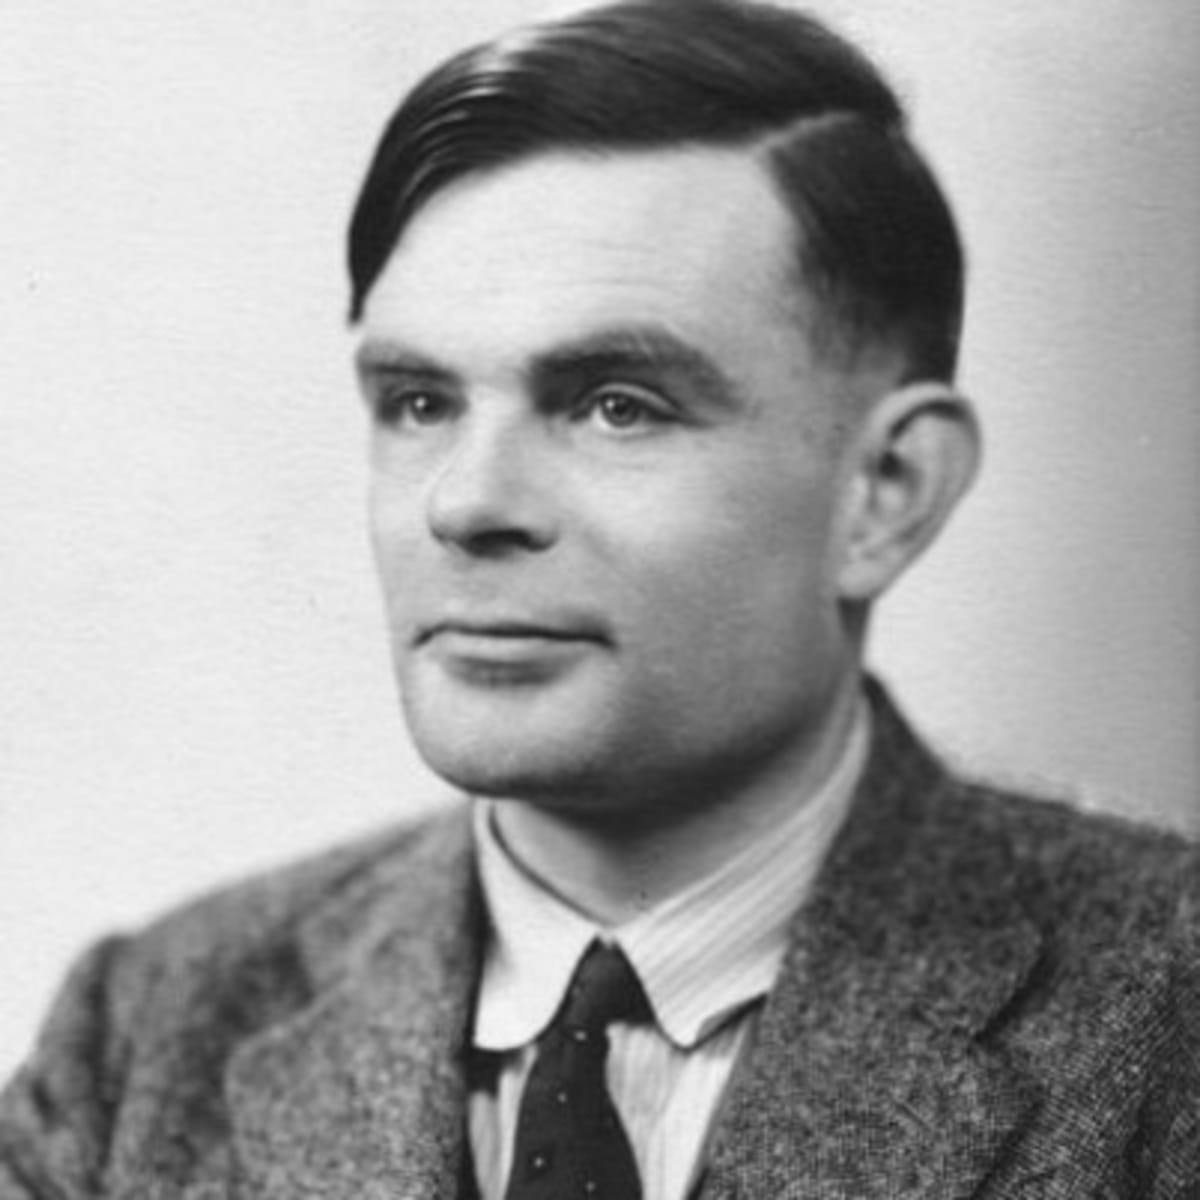
\includegraphics[width = 0.6\textwidth]{../images/alan_turing_npg_cc.jpg}
\caption{Alan Turing in 1951. © National Portrait Gallery, London.}
\label{fig:alan_turing_npg_cc}
\end{figure}

Turing was a genius cryptographer who helped break several German ciphers during World War II. But his most famous scientific contribution was a 1936 paper in which he introduced what has come to be known as a \textdef{Turing machine}{Turing machine}{FILL IN}. This hypothetical computer consists of an infinitely long tape of cells and a reader that can read one cell at a time. Each cell consists of only a single number, and the machine can move one cell at a time, reading and rewriting cells according to a finite collection of internal rules.

Turing's major insight was that this simple machine is nevertheless powerful. Nearly a century after his work, any task that can be performed by a computer --- even the world's most largest supercomputer --- could be implemented by a Turing machine, which Joseph Weizenbaum called nothing more than ``pebbles on toilet paper''.

Two years before his untimely demise in 1954, Turing published his only paper on biochemistry, which addressed the question: “Why do zebras have stripes?”

Turing was not asking why zebras have \textit{evolved} to have stripes --- this question was unsolved in Turing's time, and recent research has indicated that the stripes may be helpful in warding off flies. Rather, Turing was interested in what mechanism could produce the stripes that we see on a zebra's coat. And he reasoned that just as a simple machine can emulate a computer, some limited set of molecular ``rules'' could cause stripes to appear on a zebra's coat.

In this prologue, we will introduce a particle simulation model based on Turing's ideas. We will be amazed that a system built on very simple rules and even \textit{randomness} can nevertheless produce seemingly complex emergent behavior. And we will explore how this model can be tweaked to provide a hypothesis for the source of not just the zebra's stripes but also the leopard's spots.

\FloatBarrier
\phantomsection

\section{An Overview of Random Walks}
\label{sec:an_overview_of_random_walks}
\phantomsection

\subsection{Life is random}

Everything in the universe ultimately depends on the interaction of tiny particles. Yet this fundamental truth is difficult to process when our experience of existence is guided by ``macro'' phenomena.

You may feel like a single, coherent being, but you are just a skin-covered bag of trillions of cells that act largely independently. Over half of these cells aren't even yours! They correspond to bacteria that make up a couple of kilograms of your mass. What makes the whole affair even crueler is that your cellular symphony depends on the \textit{random} movement of particles.

Throughout this course, we will see that just because a system is driven by randomness and simple rules does not mean that it cannot have emergent behavior that is complex and elegant. Just like you.

\FloatBarrier
\phantomsection
\subsection{The wanderlust of a randomly walking particle}

Cells are full of \textdef{proteins}{proteins}{FILL IN}, complex macromolecules that perform nearly every cellular function. If a protein could move in a straight line, then it would move at 20 kph or faster, but the cytoplasm that fills the cell is so densely packed with water molecules that the protein ping-pongs off them, frequently changing direction.

We will model the movements of a cellular particle such as a protein by a \textdef{random walk}{random walk}{FILL IN} in a two-dimensional plane. At each step, the particle moves a single unit of distance in a randomly chosen direction. The video below shows a randomly walking particle taking 1000 steps.

\texttt{NEED FIGURE HERE -- TO REPLACE VIDEO}\\

The distance that the particle wanders from its starting point may surprise you. And yet perhaps this particle is just an outlier, and the typical particle would be much more of a homebody.

\FloatBarrier
\phantomsection
\subsection{From one particle to many}

If we animate the action of many independent particles following random walks, then although some particles hug the starting point and some wind up far away, most particles steadily drift outward. The following video shows a simulation of 200 randomly walking particles.

\texttt{NEED FIGURE HERE -- TO REPLACE VIDEO}\\

In fact, although the movements of a single particle are random, we can draw conclusions about the \textit{average-case} behavior of many particles can be predicted, as the following theorem indicates.

\textdef{Random Walk Theorem}{Random Walk Theorem}{FILL IN} After \textvar{n} steps of unit length in a random walk, a particle will on average find itself a distance of approximately $\sqrt{n}$ from its origin.

\begin{note}[%
If you love mathematics and are interested in seeing a proof of this theorem, check out https://biologicalmodeling.org/assets/tex/random_walk_theorem.pdf 
]\end{note}

Our experience of the world confirms the Random Walk Theorem's statement that randomly walking particles tend to drift away from their starting point. We understand, for example, that an infected COVID-19 patient can infect many others in an enclosed space in a short time frame. To take a less macabre example, we also know that when a cake is baking in the oven at home, we will not need to wait long for wonderful smells to waft outward from the kitchen.

If you are interested in seeing how to build the random walk simulation shown in the video above, then please visit the following software tutorial. This tutorial uses \textdef{CellBlender}{CellBlender}{FILL IN}, an add-on to the popular open graphics software program  \textdef{Blender}{Blender}{FILL IN}, which allows us to create and visualize biological models. These models rely on particle-based reaction-diffusion simulations that are implemented by the program  \textdef{MCell}{MCell}{FILL IN}. We will use this software for our work in biological modeling in this prologue as well as \autoref{chapter:motifs}.

\begin{note}[%
We have designed this course so that you can appreciate the key ideas behind the biological models that we build without following software tutorials. But we also provide these tutorials so that you can explore the modeling software that we have used to generate our conclusions.
]\end{note}

\tutorial[https://biologicalmodeling.org/prologue/tutorial-random-walk]

\FloatBarrier
\phantomsection
\subsection{Brownian motion: big numbers in small spaces}

Why should scientists care about random walks? Later in this book, we will see that random walks power a simple but powerful approach that bacteria like \textit{E. coli} use to explore their environment in the hunt for food. In the next section, we will see that randomly moving particles serve can produce high-level patterns if the particles interact when they collide.

Before continuing, we will point you to a beautiful animation illustrating just how far a single randomly moving particle can travel in a relatively small amount of time. This animation, which shows a simulation of the path taken by a glucose molecule as the result of Brownian motion, starts at 6:10 of the following excellent video developed by the late Joel Stiles.

\texttt{NEED FIGURE HERE -- TO REPLACE VIDEO}\\

















\FloatBarrier
\phantomsection

\section{A Reaction-Diffusion Model Generating Turing Patterns}
\label{sec:a_reaction-diffusion_model_generating_turing_patterns}
\phantomsection

\subsection{From random walks to reaction-diffusion}

In the [previous lesson](random_walk), we introduced the model of a particle randomly walking through a medium. But what exactly do random walks have to do with Alan Turing and zebras?

Turing's insight was that remarkable high-level patterns could arise if we combine particle diffusion with a chemical reaction in which colliding particles interact with each other. Such a model is called a \textdef{reaction-diffusion system}{reaction-diffusion system}{FILL IN}, and the emergent patterns are called \textdef{Turing patterns}{Turing patterns}{FILL IN} in Turing's honor.

We will consider a reaction-diffusion system having two types of particles, \textvar{A} and \textvar{B}. The system is not explicitly a predator-prey relationship, but you may like to think of the \textvar{A} particles as prey and the \textvar{B} particles as predators for reasons that will become clear soon.

Both types of particles diffuse randomly through the plane, but the \textvar{A} particles diffuse more quickly than the \textvar{B} particles.  In the simulation that follows, we will assume that \textvar{A} particles diffuse twice as quickly as \textvar{B} particles. In terms of our random walk model, this faster rate of diffusion means that in a single ``step'', an \textvar{A} particle moves twice as far as a \textvar{B} particle.

\begin{qbox}[%
Say that we release one \textvar{A} particle and one \textvar{B} particle at the same location. If the two particles move via random walks, and the rate of diffusion of \textvar{A} is twice as fast, then on average how much farther from the origin will \textvar{A} be than \textvar{B} after \textvar{n} steps?
]\end{qbox}

We now will add some reactions to our system. The \textvar{A} particles are added into the system at some constant \textdef{feed rate}{feed rate}{FILL IN} \textvar{f}. As a result of the feed reaction, the concentration of the \textvar{A} particles increases by a constant number in each time step.

\begin{note}[%
We will work with a two-dimensional simulation, but in a three-dimensional system, the units of \textvar{f} would be in mol/L/s, which means that every second, there are \textvar{f} moles of particles added to the system for every liter of volume. (Recall from your chemistry class long ago that one mole is 6.02214076 · 10<sup>23</sup> particles, called Avogadro's number.)
]\end{note}

There is also a \textdef{kill rate}{kill rate}{FILL IN} constant \textvar{k} dictating the rate of removal of \textvar{B} particles. As a result of the kill reaction, the number of \textvar{B} particles in the system will decrease by a factor of \textvar{k} in a given time step. That is, the more \textvar{B} particles that are present, the more \textvar{B} particles will be removed.

Finally, our reaction-diffusion system includes the following reaction involving both particle types. The particles on the left side of this reaction are called \textdef{reactants}{reactants}{FILL IN} and the particles on the right side are called \textdef{products}{products}{FILL IN}.

<p><center><em>A</em> + 2<em>B</em> → 3<em>B</em></center></p>

To simulate this reaction on a particle level, if an \textvar{A} particle and two \textvar{B} particles collide with each other, then the \textvar{A} particle has some fixed probability of being replaced by a third \textvar{B} particle, which could vary based on the presence of a catalyst and the orientation of the particles. This probability directly relates to the \textit{rate} at which this reaction occurs, which is denoted \textvar{r} and also depends on the concentrations of \textvar{A} and \textvar{B} as well as their kinetic energy.

This third reaction is why we compared \textvar{A} to prey and \textvar{B} to predators, since we may like to conceptualize the reaction as two \textvar{B} particles consuming an \textvar{A} particle and producing an offspring \textvar{B} particle.

The three reactions defining our system are summarized by the figure below.



Before continuing, we call your attention to a slight difference between the feed and kill reactions. In the former, the number of \textvar{A} particles increases by a constant number in each time step. In the latter, the number of \textvar{B} particles decreases by a constant factor multiplied by the current number of \textvar{B} particles. If we were using calculus to model this system, then letting [\textvar{A}] and [\textvar{B}] denote the concentrations of the two particle types, we can write

<p><center>
<em>d</em>[<em>A</em>]/<em>dt</em> = <em>f</em>
</center></p>

and

<p><center>
<em>d</em>[<em>B</em>]/<em>dt</em> = -<em>k</em> · [<em>B</em>].
</center></p>

\FloatBarrier
\phantomsection
\subsection{Parameters are omnipresent in biological modeling}

Before building a simulation corresponding to our reaction-diffusion model, we point out that the results of the simulation can vary depending upon a few things.

A \textdef{parameter}{parameter}{FILL IN} is a variable quantity used as input to a model. Parameters are inevitable in biological modeling (and data science in general), and as we will see, changing parameters can cause major changes in the behavior of a system.

Four parameters are relevant to our reaction-diffusion system. Three of these parameters are the feed rate (\textvar{f}) of \textvar{A} particles, the kill rate of the \textvar{B} particles (\textvar{k}), and the rate of the predator-prey reaction (\textvar{r}). The final parameter of interest corresponds to the diffusion rate (i.e., speeds) of the the \textvar{B} particles. Once this diffusion rate is set, the diffusion rate of \textvar{A} particles must be twice that of the \textvar{B} particles.

We think of all these parameters as dials that we can turn, observing how the system changes as a result. For example, if we raise the diffusion rate, then the particles will be moving around and bouncing into each other more, which means that we will see more of the reaction \textvar{A} + 2\textvar{B} → 3\textvar{B}.

\begin{qbox}[%
What will happen as we increase or decrease the feed rate \textvar{f}? What about the kill rate \textvar{k}?
]\end{qbox}

The same goes for the feed and kill reactions; new \textvar{A} particles are formed, and old \textvar{B} particles are destroyed, via probabilities that are computed from reaction rates. For now, you can think of the rate of a reaction as directly related to its probability of occurring.

In the following tutorial, we will initiate our reaction-diffusion system with a uniform concentration of \textvar{A} particles spread across the grid and a tightly packed collection of \textvar{B} particles in the center of the grid. When we return from this tutorial, we will see if any high-level patterns form.

\tutorial[https://biologicalmodeling.org/prologue/turing-cellblender]

\FloatBarrier
\phantomsection
\subsection{Changing reaction-diffusion parameters produces different emergent Turing patterns}

For many parameter values, our reaction-diffusion system is not very interesting.  For example, the following animation is produced when using parameter rates in CellBlender of \textvar{f} = 1000 and \textvar{k} = 500,000.  It shows that if the kill rate is too high, then the \textvar{B} particles will die out more quickly than they can be replenished by the reaction with \textvar{A} particles, and so only \textvar{A} particles will be left. In this animation, \textvar{A} particles have been colored green, and \textvar{B} particles have been colored red.

\texttt{NEED FIGURE HERE -- TO REPLACE VIDEO}\\

On the other hand, if \textvar{f} is too high, then the increased feed rate will cause an increase in the concentration of \textvar{A} particles. However, the increased concentration of \textvar{A} particles will also cause more interactions between \textvar{A} particles and pairs of \textvar{B} particles, and so we will see an explosion in the number of predators. The following simulation has the parameters \textvar{f} = 1,000,000 and \textvar{k} = 100,000.

\texttt{NEED FIGURE HERE -- TO REPLACE VIDEO}\\

The interesting behavior in this system lies in a sweet spot of the \textvar{f} and \textvar{k} parameters. For example, consider the following visualization when \textvar{f} is equal to 100,000 and \textvar{k} is equal to 200,000. We see a very clear stripe of predators expanding outward against a background of prey, with subsequent stripes appearing at locations where there is a critical mass of predators to interact with each other.

\texttt{NEED FIGURE HERE -- TO REPLACE VIDEO}\\

When we hold \textvar{k} fixed and increase \textvar{f} to 140,000, the higher feed rate increases the likelihood of \textvar{B} particles encountering \textvar{A} particles, and so we see even more stripes of \textvar{B} particles.

\texttt{NEED FIGURE HERE -- TO REPLACE VIDEO}\\

As \textvar{f} approaches \textvar{k}, the stripe structure becomes chaotic and breaks down because there are now many clusters of \textvar{B} particles colliding and mix with each other. The following animation shows the result of raising \textvar{f} to 175,000.

\texttt{NEED FIGURE HERE -- TO REPLACE VIDEO}\\

Once \textvar{f} is equal to \textvar{k}, the stripes disappear, as shown in the video below. We might expect this to mean that the \textvar{A} and \textvar{B} particles will be uniformly mixed. Instead, we see is that after an initial outward explosion of \textvar{B} particles, the system displays a mottled background, with pockets having higher or lower concentration of \textvar{B}. Pay attention to the following video at a point late in the animation. Although the concentrations of the particles are still changing, there is much less large-scale change than in earlier videos. If we freeze the video, our eye cannot help but see patterns of red and green clusters that resemble spots, or mottling.

\texttt{NEED FIGURE HERE -- TO REPLACE VIDEO}\\

You may still be skeptical, since the patterns in the above videos do not have the concrete boundaries that we might expect of animal stripes and spots. Yet when we closely examine an animal with skin patterns, we can see that the patterns we infer on a higher level are just the net result of many individual, varied points. The figure below shows an example of this effect for zebrafish skin.

\begin{figure}[h]
\centering
\mySfFamily
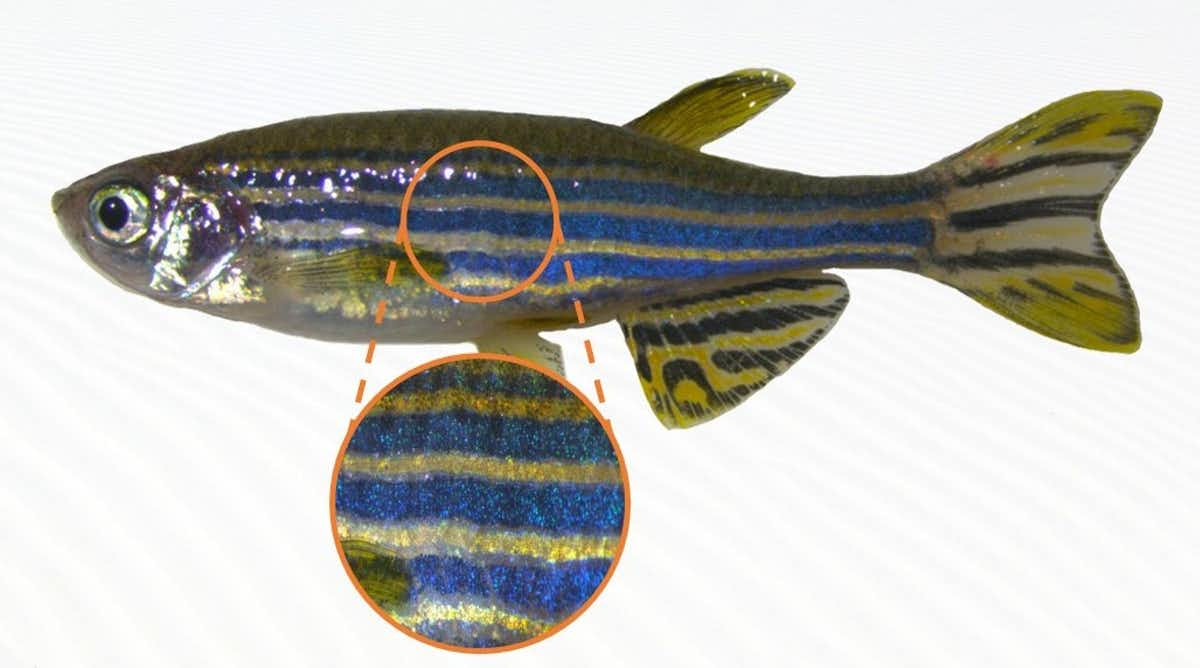
\includegraphics[width = 0.6\textwidth]{../images/zebrafish_zoom.jpg}
\caption{Zooming in on the striped skin of a zebrafish shows that each stripe is formed of thousands of differently colored cells, and that the boundaries of the stripes are more variable than they may seem at lower resolution. Image courtesy: JenniferOwen, Wikimedia Commons (adapted by Kit Yates).}
\label{fig:zebrafish_zoom}
\end{figure}

\FloatBarrier
\phantomsection
\subsection{Turing's patterns and Klüver's hallucinations}

When you watched the particle simulations above, an adjective that may have come to mind is ``trippy''. This is no accident.

Research dating all the way back to the 1920s has studied the patterns that we see during visual hallucinations, which Heinrich Klüver named \textdef{form constants}{form constants}{FILL IN} after studying patients who had taken mescaline. Form constants, such as cobwebs, tunnels, and spirals, occur across many individuals regardless of the cause of their hallucinations.

\begin{figure}[h]
\centering
\mySfFamily
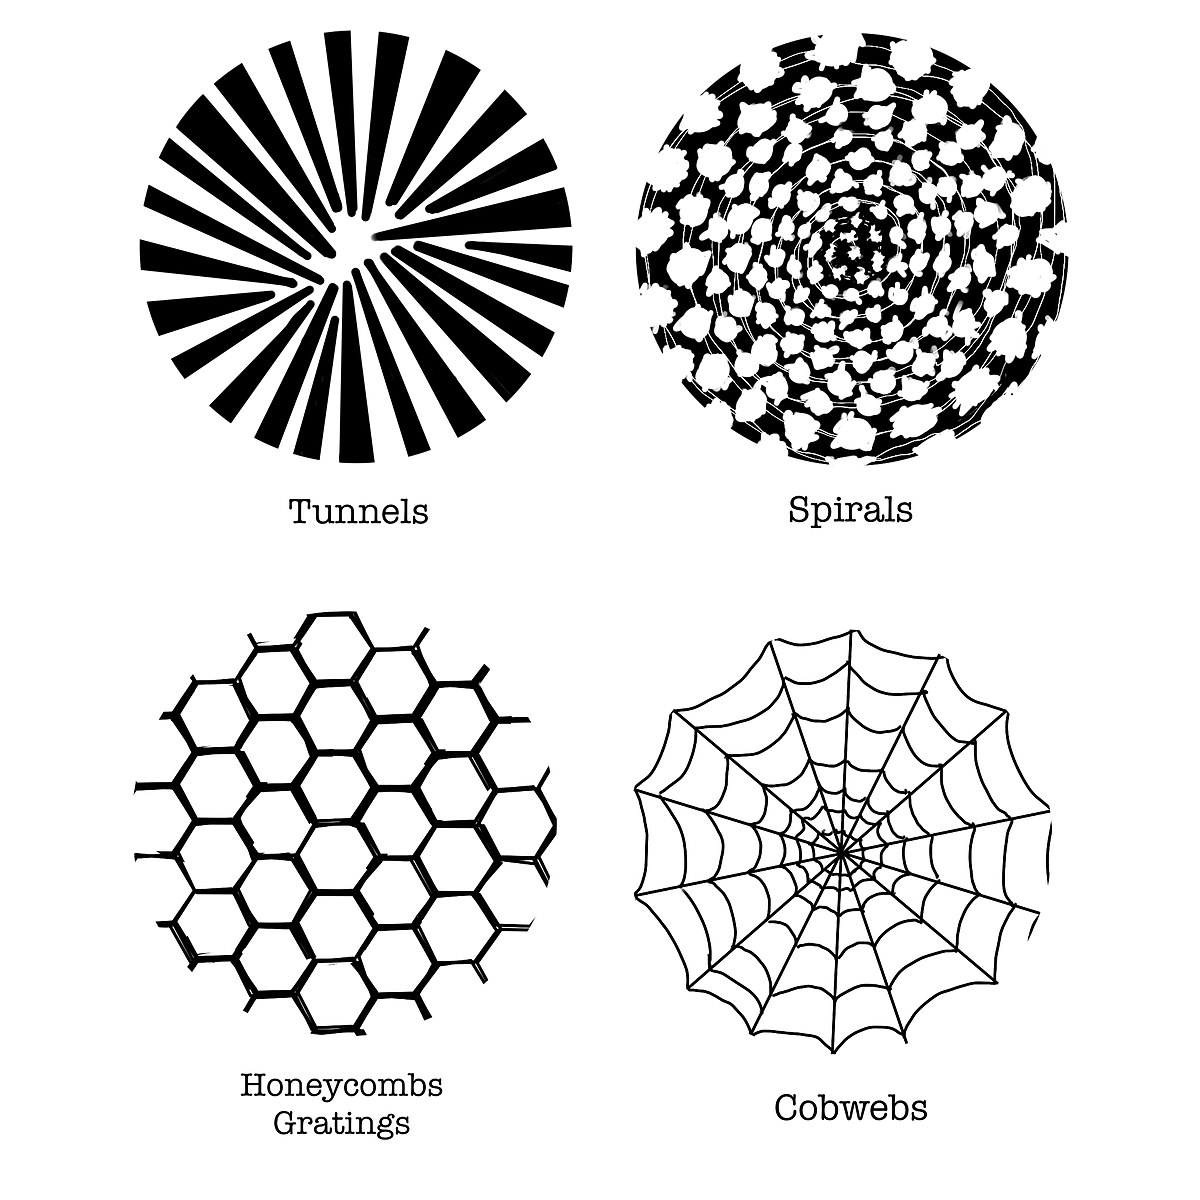
\includegraphics[width = 0.6\textwidth]{../images/form_constants.png}
\caption{A few of Heinrich Klüver's form constants. Image courtesy: Lisa Diez, Wikimedia Commons.}
\label{fig:form_constants}
\end{figure}

Over five decades after Klüver's work, researchers would determine that form constants having different shapes originate from simpler \textit{linear} stripes of cellular activation patterns in the retina. The retina is circular, but the brain needs to convert this cellular image into a rectangular field of view; as a result, when the linear patterns are passed to the visual cortex, the hallucinating brain contorts them into the spirals and whirls that we see. Some researchers believe that the patterns in the retina caused by hallucinations are in fact Turing patterns and can be explained by a reaction-diffusion model in which one type of neuron acts as a predator and another acts as prey.

\FloatBarrier
\phantomsection
\subsection{Streamlining our simulations}

Despite using advanced modeling and rendering software that has undergone years of development and optimization, each of the visualizations in this lesson took several hours to render. These simulations are computationally intensive because they require us to track the movement of tens of thousands of particles over thousands of generations.

We wonder if it is possible to build a model of Turing patterns that does not require so much computational overhead. In other words, is there a simplification that we can make to our model that will run faster but still produce Turing patterns? We will turn our attention to this question in the next lesson.





















\FloatBarrier
\phantomsection

\section{The Gray-Scott Model: A Turing Pattern Cellular Automaton}
\label{sec:the_gray-scott_model:_a_turing_pattern_cellular_automaton}
\phantomsection

\subsection{A coarse-grained model of single particle diffusion}


Part of a modeler's job is to find simple models that capture the essence of a system while running quickly and scaling well to larger inputs.

In our case, we have a very ``fine-grained'' reaction-diffusion model illustrating Turing patterns, but this model consumes a huge amount of computational resources because it requires tracking the movements of hundreds of thousands of individual particles. Our goal is to build a model that will allow us to appreciate Turing patterns without significant computational overhead.

Our idea is to grid off two-dimensional space into blocks and store only the \textit{concentration} of each type of particle found inside the block. To make things even simpler, we assume that there is some maximum concentration of particles possible, so that we can divide the number of particles by this maximum concentration. As a result, the concentration of a particle in each block will be represented by a decimal number between 0 and 1.

Let us begin with an example of the diffusion of only \textvar{A} particles; we will later add \textvar{B} particles as well as reactions to our model. Say that the particles are at maximum concentration in the central cell of our grid and are present nowhere else, as shown below.

\begin{figure}[h]
\centering
\mySfFamily
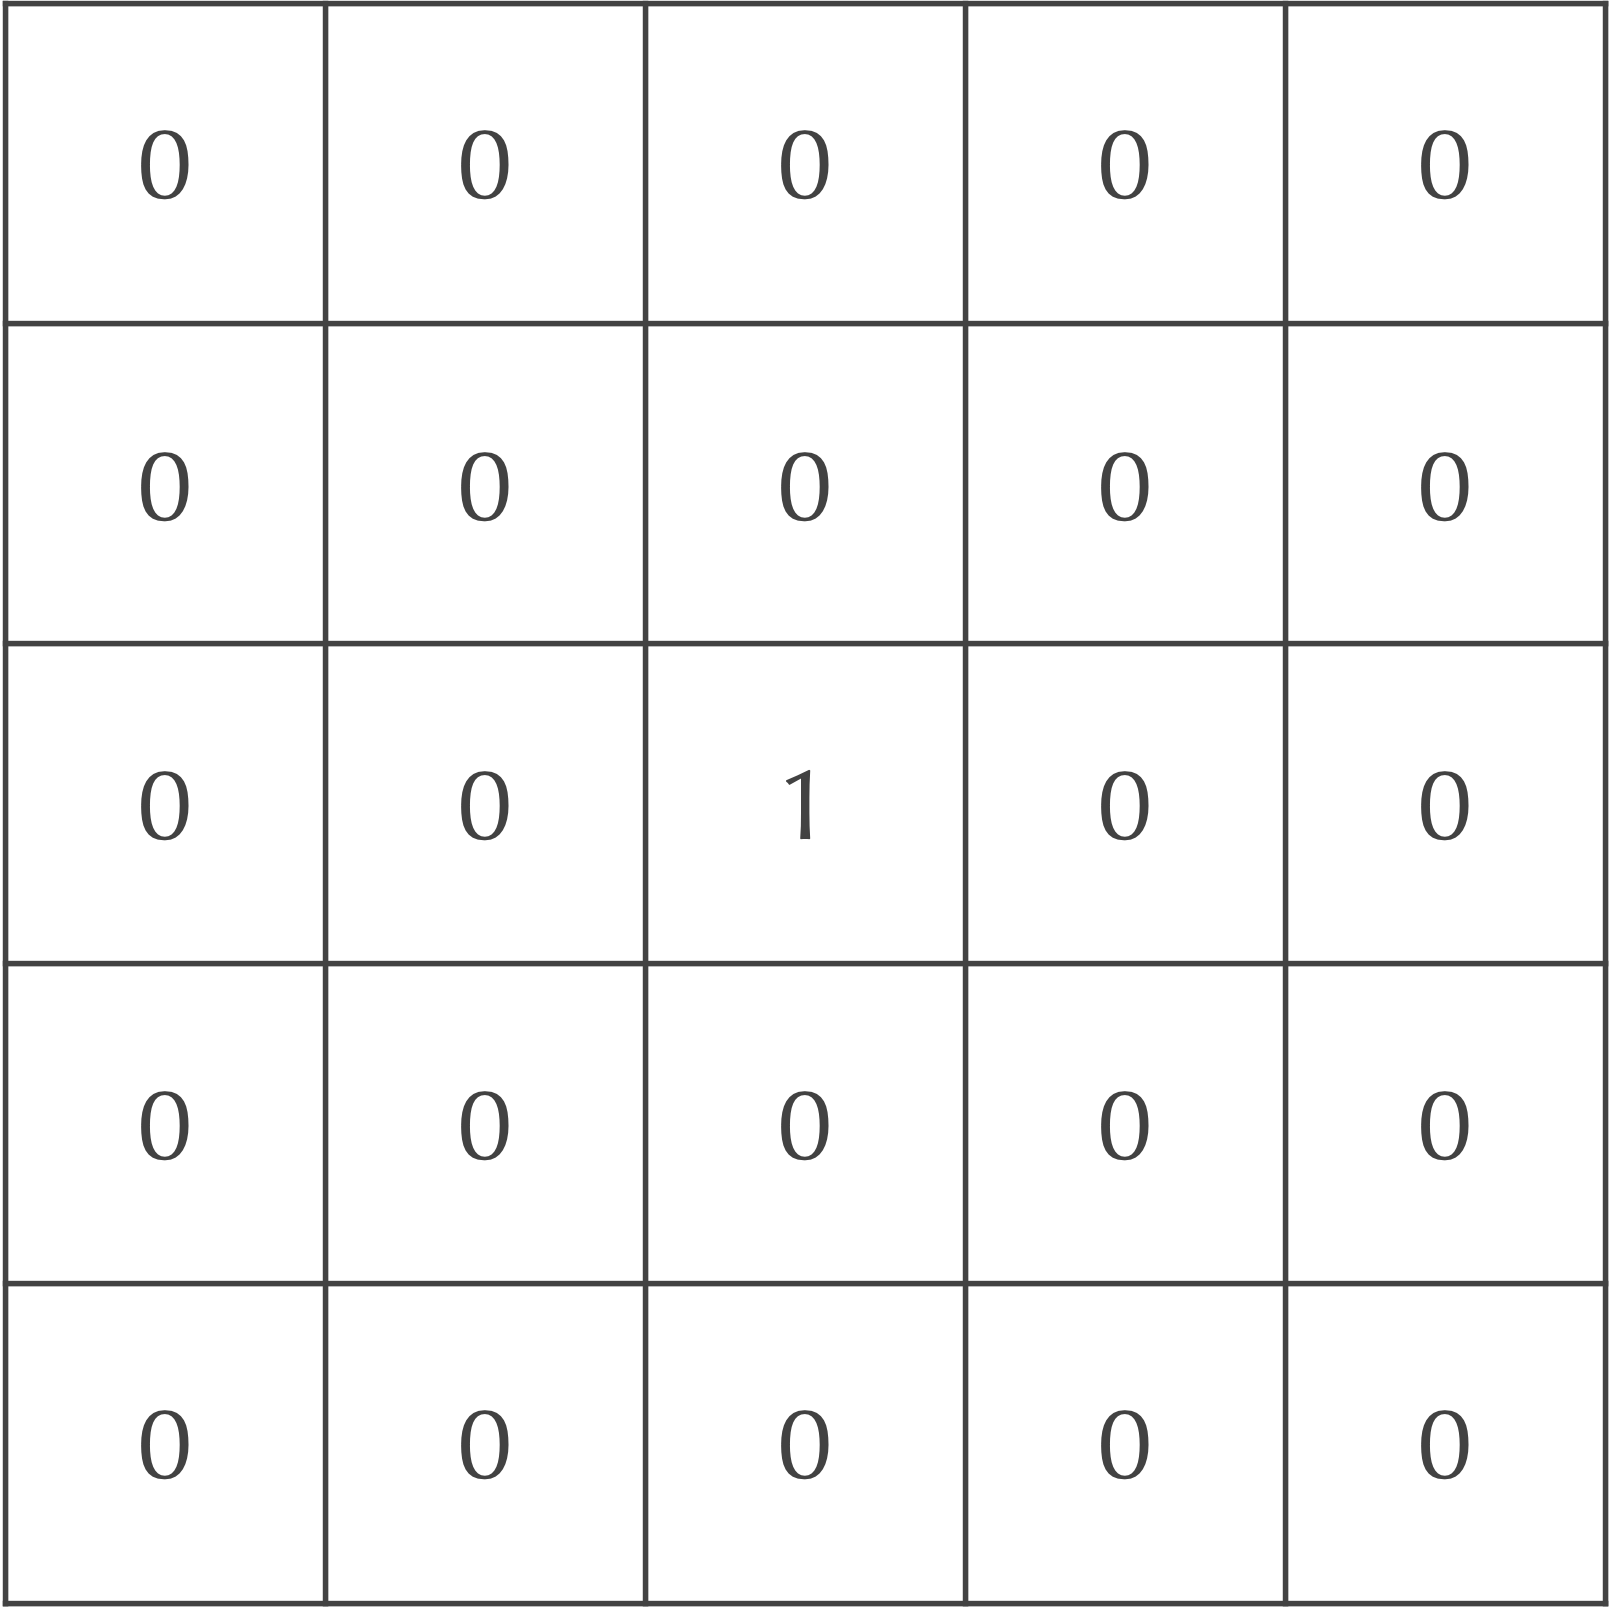
\includegraphics[width = 0.6\textwidth]{../images/initial_A_concentration.png}
\caption{A 5 x 5 grid showing hypothetical initial concentrations of \textvar{A} particles. Cells are labeled by numbers between 0 and 1 representing their concentration of \textvar{A} particles. The central cell has maximum concentration, and no particles are contained in any other cell.}
\label{fig:initial_A_concentration}
\end{figure}

We will now update the grid of cells after one time step to mimic particle diffusion. To do so, we will spread out the concentration of particles in each square to its eight neighbors. For example, we could assume that 20% of the current cell's concentration diffuses to each of its four adjacent neighbors, and that 5% of the cell's concentration diffuses to its four diagonal neighbors. Because the central square in our ongoing example is the only cell with any particles, the updated concentrations after a single time step are shown in the following figure.

\begin{figure}[h]
\centering
\mySfFamily
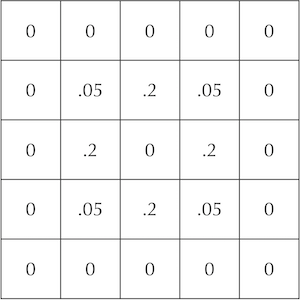
\includegraphics[width = 0.6\textwidth]{../images/A_concentration_one_time_step.png}
\caption{A grid showing an update to the system in the previous figure after diffusion of particles after a single time step.}
\label{fig:A_concentration_one_time_step}
\end{figure}

\begin{note}[%
The sum of the values in the grid in the figure above is 1, which is the same as the sum of the values in our original figure. Regardless of how many times we update the grid, the sum of the values should be 1 to ensure the conservation of total mass in the system.
]\end{note}

After an additional time step, the particles continue to diffuse outward. For example, each diagonal neighbor of the central cell in the above figure, which has a concentration of 0.05 after one time step, will lose all of its particles in the following step. Each of these cells will also gain 20% of the particles from two of its adjacent neighbors, along with 5% of the particles from the central square (which doesn't have any particles). This makes the updated concentration of this cell after two time steps equal to 2(0.2)(0.2) + 0.05(0) = 0.08.

The four cells directly adjacent to the central square, which have a concentration of 0.2 after one time step, will also gain particles from their neighbors. Each such cell will receive 20% of the particles from two of its adjacent neighbors and 5% of the particles from two of its diagonal neighbors, which have a concentration of 0.2. Therefore, the updated concentration of each of these cells after two time steps is 2(0.2)(0.05) + 2(0.05)(0.2) = 0.02 + 0.02 = 0.04.

Finally, the central square has no particles after one step, but it will receive 20% of the particles from each of its four adjacent neighbors, as well as 5% of the particles from each of its four diagonal neighbors. As a result, the central square's concentration after two time steps is 4(0.2)(0.2) + 4(0.05)(0.05) = 0.16 + 0.01 = 0.17.

In summary, the central nine squares after two time steps are as shown in the following figure.

\begin{figure}[h]
\centering
\mySfFamily
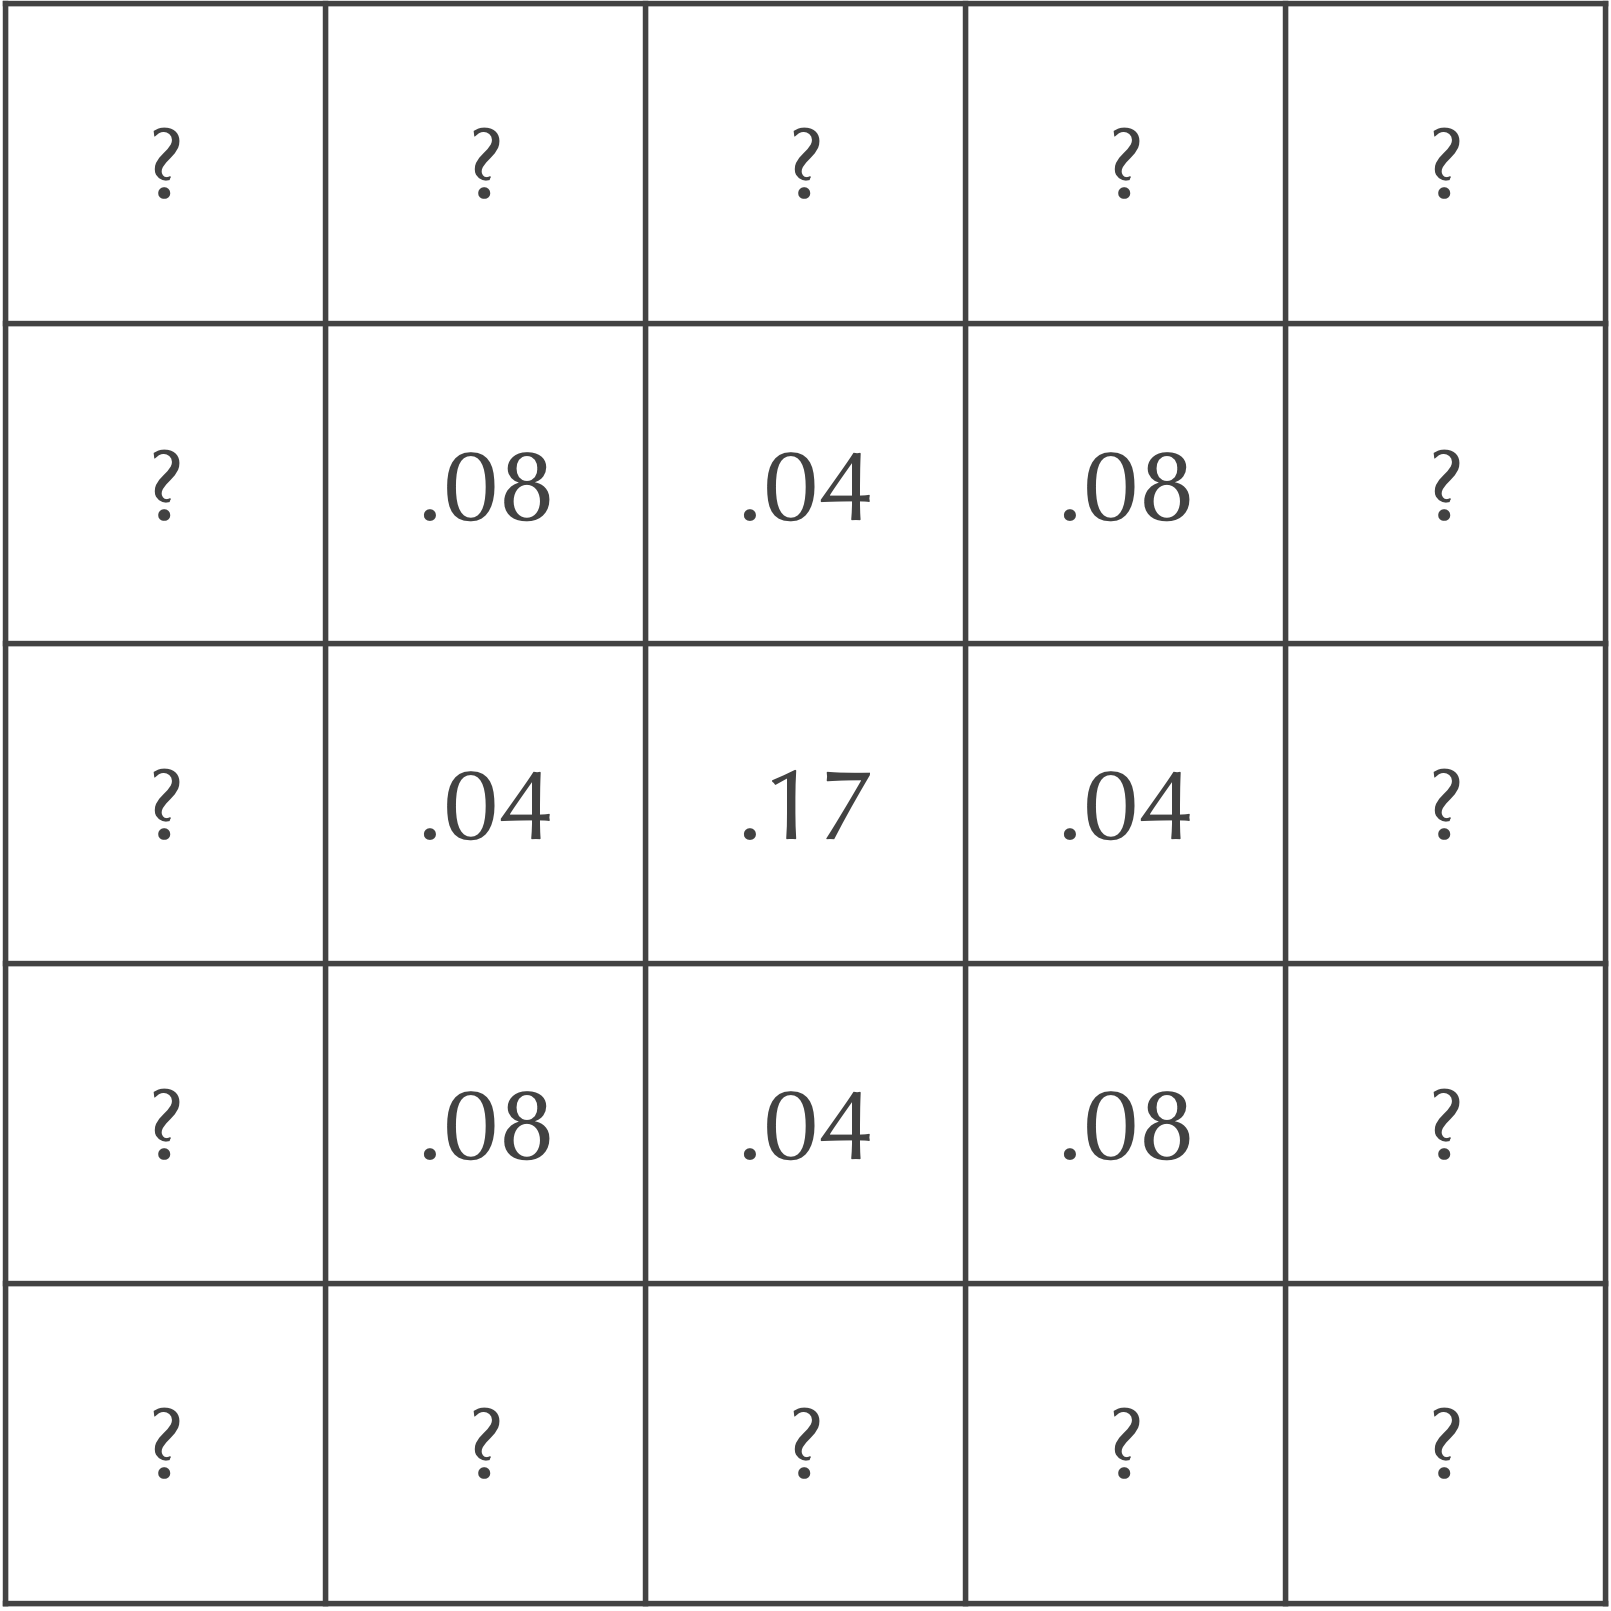
\includegraphics[width = 0.6\textwidth]{../images/A_concentration_two_time_steps_partial.png}
\caption{A grid showing an update to the central nine squares of the diffusion system in the previous figure after an additional time step. The cells labeled ``?'' are left as an exercise for the reader.}
\label{fig:A_concentration_two_time_steps_partial}
\end{figure}

\begin{qbox}[%
What should the values of the ``?'' cells be in the above figure? Note that these cells are neighbors of cells with positive concentrations after one time step, so their concentrations should be positive after two time steps.
]\end{qbox}


The coarse-grained model of particle diffusion that we have built is a variant of a \textdef{cellular automaton}{cellular automaton}{FILL IN}, or a grid of cells in which we use fixed rules to update the status of a cell based on its current status and those of its neighbors. Cellular automata form a rich area of research applied to a wide variety of fields dating back to the middle of the 20th Century; if you are interested in learning more about them from the perspective of programming, then you might like to check out the <a href="http://compeau.cbd.cmu.edu/programming-for-lovers/chapter-3-building-a-self-replicating-cellular-automaton-with-top-down-programming/" target="_blank">Programming for Lovers</a> project.

\FloatBarrier
\phantomsection
\subsection{Slowing down the rate of diffusion}

There is just one problem. Our cellular automaton model of diffusion is too volatile! The figure below shows the initial automaton as well as its updates after each of two time steps. In a true diffusion process, all of the particles would not rush out of the central square in a single time step, only for some of them to return in the next step.



Our solution is to slow down the diffusion process by adding a parameter <em>d</em><sub><em>A</em></sub> between 0 and 1 that represents the \textit{rate} of diffusion of \textvar{A} particles. Instead of moving a cell's entire concentration of particles to its neighbors in a single time step, we move only a fraction <em>d</em><sub><em>A</em></sub> of them.

Revisiting our original example, say that <em>d</em><sub><em>A</em></sub> is equal to 0.2. After the first time step, only 20% of the central cell's particles will be spread to its neighbors. Of these particles, 5% will be spread to diagonal neighbors, and 20% will be spread to adjacent neighbors. The figure below illustrates that after one time step, the central square has concentration 0.8, its adjacent neighbors have concentration 0.2<em>d</em><sub><em>A</em></sub> = 0.04, and its diagonal neighbors have concentration 0.05<em>d</em><sub><em>A</em></sub> = 0.01.

\begin{figure}[h]
\centering
\mySfFamily
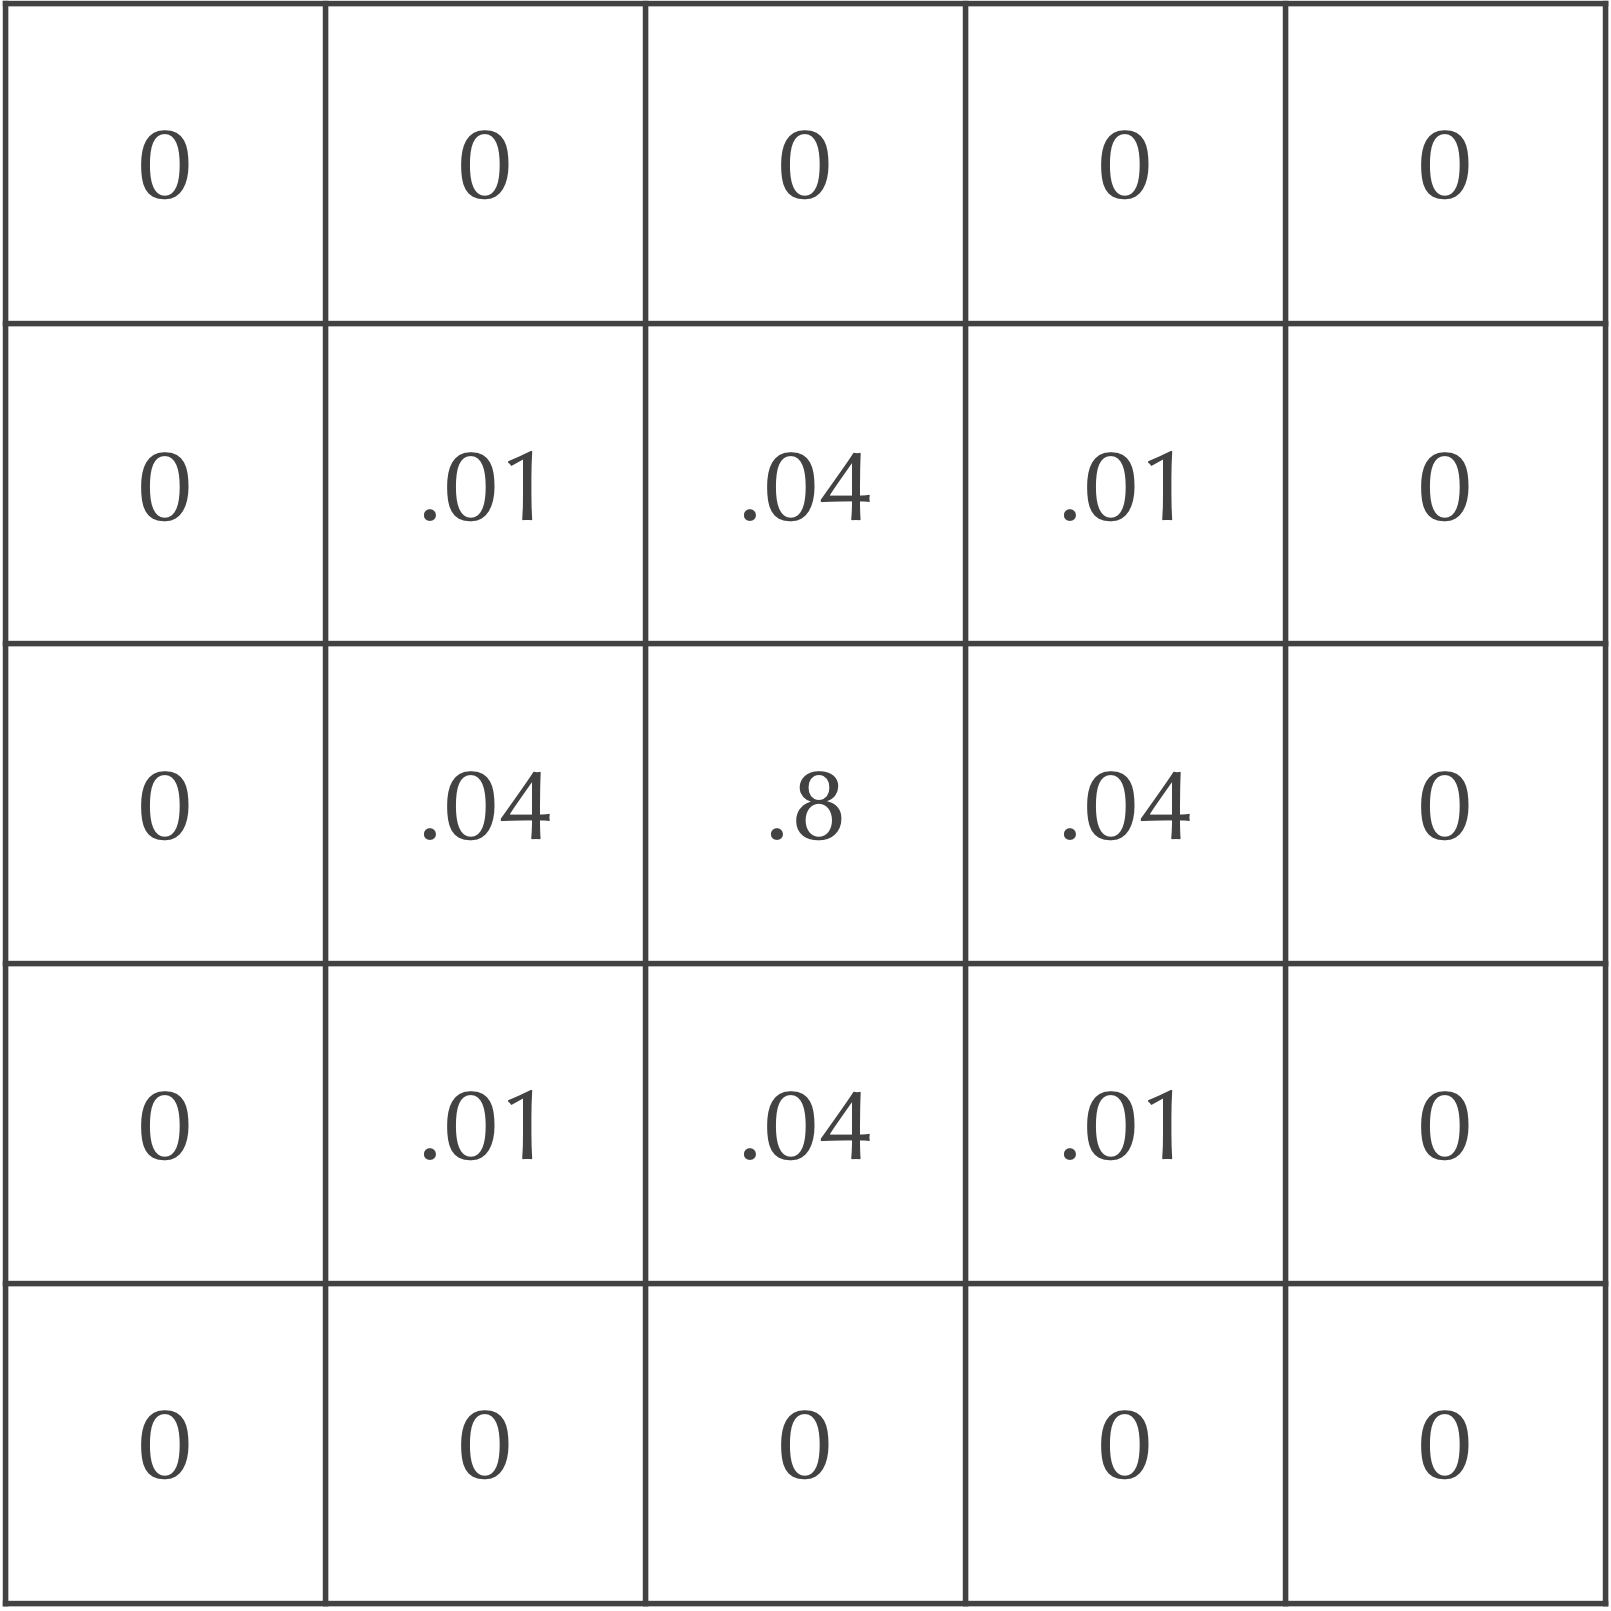
\includegraphics[width = 0.6\textwidth]{../images/A_concentration_slower_diffusion.png}
\caption{An updated grid of cells showing the concentration of <em>A</em> particles after one time step if <em>d</em><sub><em>A</em></sub> = 0.2.}
\label{fig:A_concentration_slower_diffusion}
\end{figure}

\FloatBarrier
\phantomsection
\subsection{Adding a second particle to our diffusion simulation}

We now will add particle \textvar{B} to the simulation, which also starts with 100% concentration in the central square. Recall that \textvar{B}, our "predator" molecule, diffuses half as fast as \textvar{A}, the "prey" molecule. If we set the diffusion rate <em>d</em><sub><em>B</em></sub> equal to 0.1, then our cells after a time step will be updated as shown in the figure below. This figure represents the concentration of the two particles in each cell as an ordered pair ([\textvar{A}], [\textvar{B}]).

\begin{figure}[h]
\centering
\mySfFamily
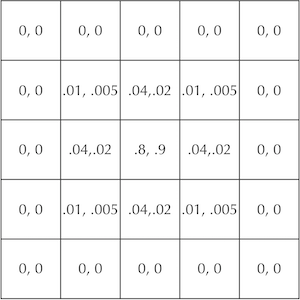
\includegraphics[width = 0.6\textwidth]{../images/two_particle_concentration_diffusion.png}
\caption{A figure showing cellular concentrations after one time step for two particles <em>A</em> and <em>B</em> diffusing at rates <em>d</em><sub><em>A</em></sub> = 0.2 and <em>d</em><sub><em>B</em></sub> = 0.1. Each cell is labeled by the ordered pair ([<em>A</em>], [<em>B</em>]).}
\label{fig:two_particle_concentration_diffusion}
\end{figure}

\begin{qbox}[%
Update the cells in the above figure after another generation of diffusion. Use the diffusion rates <em>d</em><sub><em>A</em></sub> = 0.2 and <em>d</em><sub><em>B</em></sub> = 0.1.
]\end{qbox}

\FloatBarrier
\phantomsection
\subsection{Visualizing particle concentrations}

As we move toward diffusing a large board that is hundreds of cells wide, listing the concentrations of our two particles in each cell will be too much to process. Instead, we need some way to visualize the results of our diffusion simulation.

First, we will consolidate the information stored in a cell about the concentrations of two particles into a single value. In particular, let a cell's particle concentrations be denoted [\textvar{A}] and [\textvar{B}]. Then the single value [\textvar{B}]/([\textvar{A}] + [\textvar{B}]) is the ratio of the concentration of \textvar{B} particles to the total number of particles in the cell. This value ranges between 0 (no \textvar{B} particles present) and 1 (only \textvar{B} particles present).

Next, we color each cell in the grid according to its value of [\textvar{B}]/([\textvar{A}] + [\textvar{B}]) using a color spectrum like those shown in the figure below. We will use the `Spectral` color map, meaning that if a cell has a value close to 0 (relatively few predators), then it will be colored red, while if it has a value close to 1 (relatively many predators), then it will be colored dark blue.

\begin{figure}[h]
\centering
\mySfFamily
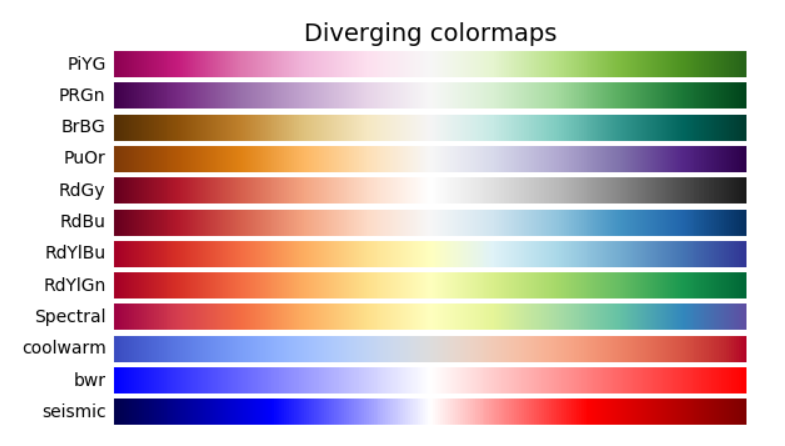
\includegraphics[width = 0.6\textwidth]{../images/matplotlib_colormap.png}
\caption{}
\label{fig:matplotlib_colormap}
\end{figure}

When we color each cell over many time steps, we can animate the automaton to see how it changes over time. We are now ready for the following tutorial, in which we will implement and visualize our diffusion automaton using a \textdef{Jupyter notebook}{Jupyter notebook}{FILL IN}.

\tutorial[https://biologicalmodeling.org/prologue/tutorial-diffusion]

The video below shows an animation of a 101 x 101 board that begins with the following properties:
\begin{itemize}
\item [\textvar{A}] = 1 for all cells;
\item [\textvar{B}] = 0 for all cells other than an 11 x 11 square in the middle of the grid, where [\textvar{B}] = 1;
\item <em>d</em><sub><em>A</em></sub> = 0.5;
\item <em>d</em><sub><em>B</em></sub> = 0.25.
\end{itemize}

\begin{figure}[h]
\centering
\mySfFamily

\includegraphics[width = 0.6\textwidth]{../images/diffusion_movie_first_frame.png}
\caption{}
\label{fig:diffusion_movie_first_frame}
\end{figure}

Note that the center of the cell becomes blue because the \textvar{A} particles diffuse twice as fast, so that they spread out more from the middle of the board, which is occupied in greater numbers by \textvar{B} particles.

\FloatBarrier
\phantomsection
\subsection{Adding reactions to our automaton: the Gray-Scott model}

Now that we have established a cellular automaton for coarse-grained particle diffusion, we will add to it the three reactions that we introduced in the [previous lesson](reaction-diffusion), which are reproduced below.

\begin{enumerate}
\item A ``feed'' reaction in which new \textvar{A} particles are fed into the system at a constant rate.
\item A ``death'' reaction in which \textvar{B} particles are removed from the system at a rate proportional to their current concentration.
\item A ``reproduction'' reaction \textvar{A} + 2\textvar{B} → 3\textvar{B}.
\end{enumerate}

\begin{qbox}[%
How might we incorporate these reactions into our automaton?
]\end{qbox}

We will address these reactions one at a time. First, we have the feed reaction, which takes place at a rate \textvar{f}. It is tempting to simply add some constant value \textvar{f} to the concentration of each cell in each time step. However, if [\textvar{A}] were close to 1, then adding \textvar{f} to it could cause [\textvar{A}] to exceed 1, which we should avoid.

Instead, if a cell has current concentration [\textvar{A}], then we will add \textvar{f}(1-[\textvar{A}]) to this cell's concentration of \textvar{A} particles. For example, if [\textvar{A}] is 0.01, then we will add 0.99\textvar{f} to the cell because the current concentration is low. If [\textvar{A}] is 0.8, then we will only add 0.2\textvar{f} to the concentration.

Second, we consider the death reaction of \textvar{B} particles, which takes place at rate \textvar{k}. Recall from the previous lesson that \textvar{k} is proportional to the current concentration of \textvar{B} particles. As a result, if a cell has concentration [\textvar{B}], then for some constant \textvar{k} between 0 and 1, we will subtract \textvar{k} · [\textvar{B}] from the current concentration of \textvar{B} particles.

Third, we have the reproduction reaction \textvar{A} + 2\textvar{B} → 3\textvar{B}, which takes place at a rate \textvar{r}. The higher the concentration of \textvar{A} and \textvar{B}, the more this reaction will take place. Furthermore, because we need \textit{two} \textvar{B} particles in order for the collision to occur, the reaction should be even more rare if we have a low concentration of \textvar{B} than if we have a low concentration of \textvar{A}. To model this situation, if a given cell is represented by the concentrations ([\textvar{A}], [\textvar{B}]), then we will subtract \textvar{r} · [\textvar{A}] · [\textvar{B}]<sup>2</sup> from the concentration of \textvar{A} and add \textvar{r} · [\textvar{A}] · [\textvar{B}]<sup>2</sup> to the concentration of \textvar{B} in the next time step.

In summary, say that a cell has current concentrations [\textvar{A}] and [\textvar{B}]. Say also that as the result of diffusion, the change in its concentrations are Δ\textvar{A} and Δ\textvar{B}, where a negative number represents particles leaving the cell, and a positive number represents particles entering the cell. Then in the next time step, the particle concentrations [\textvar{A}]<sub>new</sub> and [\textvar{B}]<sub>new</sub> are given by the following equations.

[\textvar{A}]<sub>new</sub> = [\textvar{A}] + Δ\textvar{A} +  \textvar{f}(1-[\textvar{A}]) - \textvar{r} · [\textvar{A}] · [\textvar{B}]<sup>2</sup>
[\textvar{B}]<sub>new</sub> = [\textvar{B}] + Δ\textvar{B} - \textvar{k} · [\textvar{B}] + \textvar{r} · [\textvar{A}] · [\textvar{B}]<sup>2</sup>

Applying these reaction-diffusion computations over all cells in parallel and over many generations forms a cellular automaton called the \textdef{Gray-Scott}{Gray-Scott}{FILL IN} model.

Before continuing, let us consider an example of how a single cell might update its concentration of both particle types as a result of reaction and diffusion.  Say that we have the following hypothetical parameter values:

\begin{itemize}
\item <em>d</em><sub><em>A</em></sub> = 0.2;
\item <em>d</em><sub><em>B</em></sub> = 0.1;
\item \textvar{f} = 0.3;
\item \textvar{k} = 0.4;
\item \textvar{r} = 1 (the value typically always used in the Gray-Scott model).
\end{itemize}

Furthermore, say that our cell has the concentrations ([\textvar{A}], [\textvar{B}]) = (0.7, 0.5). Then as a result of diffusion, the cell's concentration of \textvar{A} will decrease by 0.7 · <em>d</em><sub><em>A</em></sub> = 0.14, and its concentration of \textvar{B} will decrease by 0.5 · <em>d</em><sub><em>B</em></sub> = 0.05. It will also receive particles from neighboring cells; for example, say that it receives an increase to its concentration of \textvar{A} by 0.08 and an increase to its concentration of \textvar{B} by 0.06 as the result of diffusion from neighbors. Therefore, Δ\textvar{A} = 0.08 - 0.14 = -0.06, and Δ\textvar{B} = 0.06 - 0.05 = 0.01.

Now we will consider the three reactions. The feed reaction will cause the cell's concentration of \textvar{A} to increase by (1 - [\textvar{A}]) · \textvar{f} = 0.09. The death reaction will cause its concentration of \textvar{B} to decrease by \textvar{k} · [\textvar{B}] = 0.2. And the reproduction reaction will mean that the concentration of \textvar{A} decreases by [\textvar{A}] · [\textvar{B}]<sup>2</sup> = 0.175, with the concentration of \textvar{B} increasing by the same amount.

As the result of all these processes, we update the concentrations of \textvar{A} and \textvar{B} to the following values ([\textvar{A}]<sub>new</sub>, [\textvar{B}]<sub>new</sub>) in the next time step according to our equations above.

[\textvar{A}]<sub>new</sub> = 0.7 - 0.06 + 0.09 - 0.175 = 0.555<br>
[\textvar{B}]<sub>new</sub> = 0.5 + 0.01 - 0.2 + 0.175 = 0.485

We should now feel ready to implement the Gray-Scott model in the following tutorial. The question is: even though we have built a coarser-grained simulation than the previous lesson, will we still see Turing patterns?

\tutorial[https://biologicalmodeling.org/prologue/gs-jupyter]

\FloatBarrier
\phantomsection
\subsection{Reflection on the Gray-Scott model}

In contrast to our particle-based simulator, the Gray-Scott model produced an animation of Turing patterns in under a minute on a laptop. We show the results of this model in the videos that follow; throughout these animations, we use the parameters <em>d</em><sub><em>A</em></sub> = 1.0, <em>d</em><sub><em>B</em></sub> = 0.5, and \textvar{r} = 1.

Our first video shows an animation of the Gray-Scott model using the parameters \textvar{f} = 0.034 and \textvar{k} = 0.095. We use the same initial configuration of the automaton that we used in the diffusion example, in which a cluster of \textvar{B} particles are found at the middle of a board full of \textvar{A} particles.

\begin{figure}[h]
\centering
\mySfFamily

\includegraphics[width = 0.6\textwidth]{../images/gray-scott_movie_first_frame.png}
\caption{}
\label{fig:gray-scott_movie_first_frame}
\end{figure}

If we expand the size of the simulation and add multiple clusters of predators to the automaton, then the patterns become more complex as they intersect.

\begin{figure}[h]
\centering
\mySfFamily

\includegraphics[width = 0.6\textwidth]{../images/gray-scott_multiple_predators_first_frame.png}
\caption{}
\label{fig:gray-scott_multiple_predators_first_frame}
\end{figure}

If we keep the feed rate constant and increase the kill rate slightly to \textvar{k} = 0.097, then the patterns change significantly into spots.

\begin{figure}[h]
\centering
\mySfFamily

\includegraphics[width = 0.6\textwidth]{../images/gray-scott_f34_k63_first_frame.png}
\caption{}
\label{fig:gray-scott_f34_k63_first_frame}
\end{figure}

If we make the prey a little happier as well, increasing  \textvar{f} to 0.038 and \textvar{k} to 0.099, then we have a different striped pattern.

\begin{figure}[h]
\centering
\mySfFamily
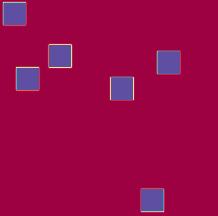
\includegraphics[width = 0.6\textwidth]{../images/gray-scott_f38_k61_first_frame.png}
\caption{}
\label{fig:gray-scott_f38_k61_first_frame}
\end{figure}

And if we increase \textvar{f} to 0.042 and \textvar{k} to 0.101, then again we see spots.

\begin{figure}[h]
\centering
\mySfFamily

\includegraphics[width = 0.6\textwidth]{../images/gray-scott_f42_k59_first_frame.png}
\caption{}
\label{fig:gray-scott_f42_k59_first_frame}
\end{figure}

The point is that very slight changes in our model's parameters can produce drastically different results in terms of the patterns that we witness. In this prologue's conclusion, we will connect this observation back to our original motivation of identifying the cause for animal skin patterns.



















\FloatBarrier
\phantomsection

\section{Conclusion: Turing Patterns are Fine-Tuned}
\label{sec:conclusion:_turing_patterns_are_fine-tuned}
\phantomsection


The Turing patterns that emerged from our particle simulations are a testament to the human eye's ability to find organization within the net behavior of tens of thousands of particles. For example, take another look at the video we produced that showed mottling in our particle simulator. Patterns are present, but they are also noisy --- even in the dark red regions we will have quite a few green particles, and vice-versa. The rapid inference of large-scale patterns from small-scale visual phenomena is one of the tasks that our brains have evolved to perform well.

\texttt{NEED FIGURE HERE -- TO REPLACE VIDEO}\\

Our reaction-diffusion system is remarkable because it is so \textdef{fine-tuned}{fine-tuned}{FILL IN}, meaning that very slight changes in parameter values can lead to significant changes in the system. These changes could convert spots to stripes, or they could influence how clearly defined the boundaries of the Turing patterns are.

The figure below shows how the Turing patterns produced by the Gray-Scott model change as the kill and feed rates vary. The kill rate increases along the x-axis, and the feed rate increases along the y-axis. Notice how much the patterns change! You may like to tweak the parameters of the own Gray-Scott simulation from the [previous lesson](gray-scott) to see if you can reproduce these differing patterns.

\begin{figure}[h]
\centering
\mySfFamily
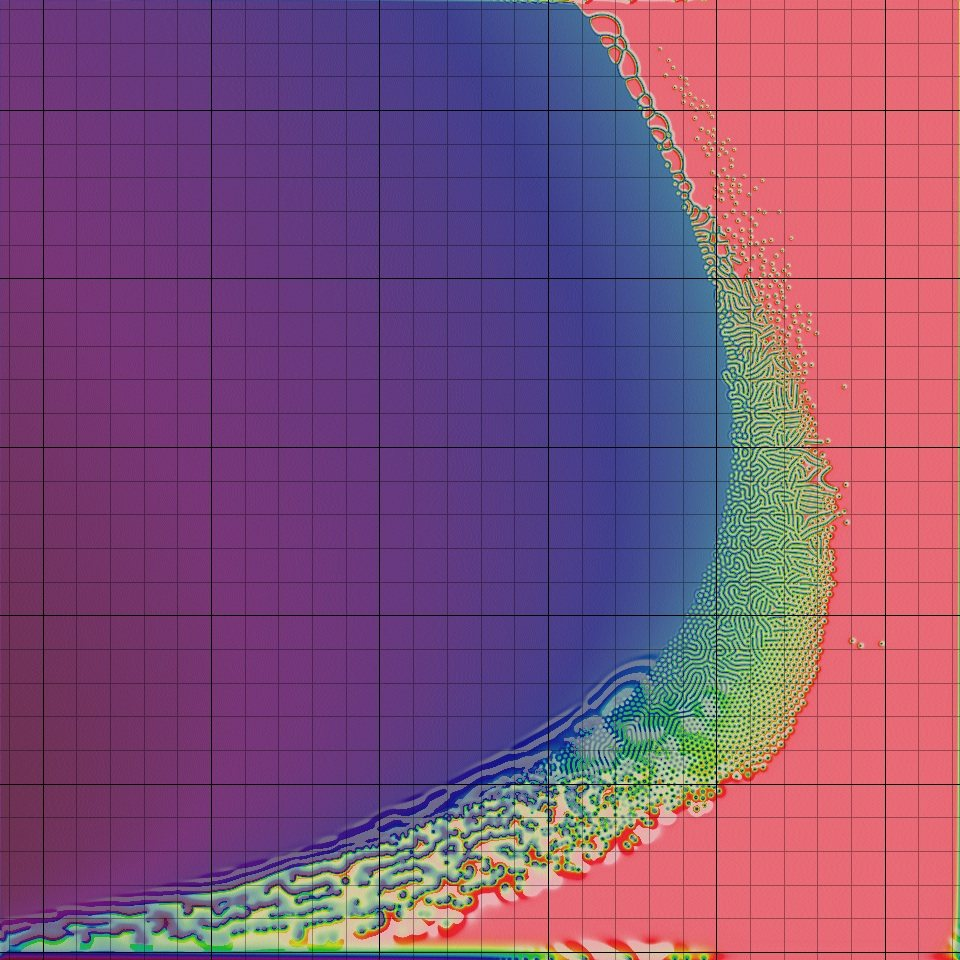
\includegraphics[width = 0.6\textwidth]{../images/xmorphia-parameter-map.jpg}
\caption{Changing kill (x-axis) and feed (y-axis) parameters greatly affects the Turing patterns produced in the Gray-Scott model. Note that many parameter choices do not lead to patterns. Image courtesy: Robert Munafo.}
\label{fig:xmorphia-parameter-map}
\end{figure}

Later in this course, we will see an example of a biological system that is the opposite of fine-tuned. In a \textdef{robust}{robust}{FILL IN} system, variation in parameters does not lead to substantive changes in the ultimate behavior of the system. Robustness is vital for processes, like your heartbeat, that must be resilient to small environmental changes.

It turns out that although Turing's work offers a compelling argument for how zebras might have gotten their stripes, the exact mechanism causing these stripes to form is still an unresolved question. However, the skin of \textit{zebrafish} does exhibit Turing patterns because two types of pigment cells follow a reaction-diffusion model much like the one we presented in this prologue. This prologue presented Turing particles as driven by the interactions of particles, but if the interactions occur between cells, then the resulting patterns are the same.

Finally, take a look at the following two photos of giant pufferfish. These fish are genetically practically identical, but their skin patterns are very different. What may seem like a drastic change from spots to stripes is likely attributable to a small change of parameters in a fine-tuned biological system that, like much of life, is powered by randomness.








